%! Author = gabriel
%! Date = 3/18/22

% Preamble
\documentclass[12pt]{beamer}

% Packages
\usepackage{amsmath}
\usepackage{pgfplots}
\usepackage{minted}
\usepackage[utf8]{inputenc}
\usepackage{hyperref}
\usepackage{tikz}
\usepackage{braket}
\usepackage{svg}
\usepackage{xcolor}

\usetheme{Madrid}
\usecolortheme[named=darkgray]{structure}
\setbeamercolor{background canvas}{bg=gray}
%\setbeamercolor{frametitle}{bg=darkgray}
\setbeamercolor{footline}{bg=darkgray}
\setbeamertemplate{enumerate items}[default]
%\setbeamercolor{titlelike}{fg=white}
%\usefonttheme{structuresmallcapsserif}
\usefonttheme{serif}
\title{Algoritmo de Grover: \\ Ket vs Qiskit}
\author{\href{https://github.com/G-Carneiro}{Gabriel Carneiro}}
%\institute[UFSC]{Universidade Federal de Santa Catarina}
%\date{\today}

\setminted[python]{
    breaklines,
    fontsize=\scriptsize,
    linenos
}

\titlegraphic{
    
\includegraphics[scale=0.15]{vertical_extenso_PB_fundo_claro}
}

\setbeamertemplate{title page}[default][rounded=true]
\setbeamertemplate{footline}{
    \leavevmode%
    \hbox{%
        \begin{beamercolorbox}[wd=0.7\paperwidth,ht=2.25ex,dp=1ex,leftskip=1em]{footline}%
            
\includegraphics[scale=0.05]{vertical_sigla_PB_fundo_claro}\hspace*{1em}%
            \usebeamerfont{author in head/foot}\insertshortauthor
        \end{beamercolorbox}%
%        \begin{beamercolorbox}[wd=.3\paperwidth,ht=2.25ex,dp=1ex,center]{title in head/foot}%
%            \usebeamerfont{title in head/foot}\insertshorttitle
%        \end{beamercolorbox}%
        \begin{beamercolorbox}[wd=.3\paperwidth,ht=2.25ex,dp=1ex,right]{date in head/foot}%
%            \usebeamerfont{date in head/foot}\insertshortdate{}\hspace*{2em}
            \insertframenumber{} / \inserttotalframenumber\hspace*{2ex}
        \end{beamercolorbox}}%
    \vskip0pt%
}

\newcommand{\precision}[2]{
\begin{tikzpicture}
    \begin{axis}[
        x tick label style={/pgf/number format/1000 sep=},
        ybar,
        bar width = 7pt,
        xmin=#1,
        xmax=#2,
        ymin=0.9,
        xlabel={Nº Qubits},
        ylabel={Precisão},
        legend entries={qubox, local, qubox-pbwd, qiskit-aer},
        enlargelimits=0.15,
        legend style={at={(0.5,-0.2)},anchor=north,legend columns=-1}
    ]
        \addplot table [x=qubits, y=precision] {dat/grover/ket_qubox_01.dat};
        \addplot table [x=qubits, y=precision] {dat/grover/ket_local_01.dat};
        \addplot table [x=qubits, y=precision] {dat/grover/ket_qubox_pbwd_01.dat};
        \addplot table [x=qubits, y=precision] {dat/grover/qiskit_aer_01.dat};
    \end{axis}
\end{tikzpicture}
}

% TODO: inserir link para simulador

\begin{document}
    \begin{frame}[plain]
        \titlepage
    \end{frame}

    \begin{frame}{Problema}
        Encontrar determinado elemento em uma lista desordenada de tamanho $2^n$.

        \[
            f(x) =
            \begin{cases}
                0, x \ne x_0 \\
                1, x = x_0
            \end{cases}
        \]

        Cada elemento da lista será codificado em um estado da base computacional.
    \end{frame}

    \begin{frame}{Algoritmo}
        \begin{enumerate}
            \item $H^{\otimes n} \ket{0}^{\otimes n}$
            \item Aplicar operador de Grover $G$ $k$ vezes:
            \begin{enumerate}
                \item Aplicar oráculo;
                \item Aplicar a porta de Hadamard em todos os qubits;
                \item Aplicar o operador $2 \ket{0}\bra{0} - I$;
                \item Aplicar a porta de Hadamard em todos os qubits.
            \end{enumerate}
        \end{enumerate}
    \end{frame}

    \begin{frame}{Notação Auxiliar}
        \[
        \begin{matrix}
            \mathbb{B}_n: \text{conjunto de todas as palavras de n bits}. \\
            \mathbb{M}: \text{conjunto de todos itens desejados}. \\
            N = 2^n
            \begin{cases}
                n: \text{número de qubits}. \\
                N: \text{número de itens}.
            \end{cases} \\
            M: \text{número de itens desejados}. \\
            \ket{\alpha} := \displaystyle \sum_{\substack{x \in \mathbb{B}_n \\ f(x) = 0}} \frac{\ket{x}}{\sqrt{N - M}} \\
            \ket{\beta} := \displaystyle \sum_{\substack{x \in \mathbb{B}_n \\ f(x) = 1}} \dfrac{\ket{x}}{\sqrt{M}} : \text{itens desejados}. \\
            S := \text{span}_\mathbb{R} \{ \ket{\alpha}, \ket{\beta} \}.
        \end{matrix}
        \]
    \end{frame}

    \begin{frame}{Primeira Aplicação de $G$}
        \[
        \begin{matrix}
            \ket{\psi_0} &=& \ket{+}^{\otimes n} \\
            &=& \displaystyle\sum_{x \in \mathbb{B}_n} \dfrac{\ket{x}}{\sqrt{N}} \\
            &=& \displaystyle\sum_{\substack{x \in \mathbb{B}_n \\ x \ne x_0}}\dfrac{\ket{x}}{\sqrt{N}} + \dfrac{\ket{x_0}}{\sqrt{N}} \\
            &=& \dfrac{\sqrt{N - 1}}{\sqrt{N}}\displaystyle\sum_{\substack{x \in \mathbb{B}_n \\ x \ne x_0}}\dfrac{\ket{x}}{\sqrt{N - 1}} + \dfrac{\ket{x_0}}{\sqrt{N}} \\
            &=& \dfrac{\sqrt{N - 1}}{\sqrt{N}} \ket{\alpha} + \dfrac{1}{\sqrt{N}} \ket{\beta}
        \end{matrix}
        \]
    \end{frame}

    \begin{frame}{Primeira Aplicação de $G$: Oráculo}
        \begin{columns}
        \column{0.5\textwidth}
        \[
        \begin{matrix}
            \ket{\psi_1} &=& O_F \ket{\psi_0} \\
            &=& \dfrac{\sqrt{N - 1}}{\sqrt{N}} \ket{\alpha} - \dfrac{1}{\sqrt{N}} \ket{\beta}
        \end{matrix}
        \]

        \column{0.5\textwidth}
        \begin{figure}
            \includesvg[scale=0.7]{figures/oracle_application}
            \caption{Oráculo equivale a uma reflexão em relação ao eixo $\ket{\alpha}$.}
            \label{fig:oracle}
        \end{figure}
        \end{columns}
    \end{frame}

    \begin{frame}{Primeira Aplicação de $G$: Difusor}
        \only<1-2>{
        \[
        \tiny
        \begin{matrix}
            2 \left| 0 \right\rangle \left\langle 0 \right| - I &=& 2 \cdot
            \begin{bmatrix}
                1       \\
                0       \\
                \vdots  \\
                0
            \end{bmatrix}_{n \times 1}
            \begin{bmatrix}
                1 & 0 & \cdots & 0
            \end{bmatrix}_{1 \times n} -
            \begin{bmatrix}
                1 & 0 & \cdots & 0 \\
                0 & 1 & \cdots & 0 \\
                \vdots & \vdots & \ddots & 0 \\
                0 & 0 & \cdots & 1
            \end{bmatrix}_{n \times n}
            \\ \\
            &=&
            \begin{bmatrix}
                2 & 0 & \cdots & 0 \\
                0 & 0 & \cdots & 0 \\
                \vdots & \vdots & \ddots & 0 \\
                0 & 0 & \cdots & 0
            \end{bmatrix}_{n \times n} -
            \begin{bmatrix}
                1 & 0 & \cdots & 0 \\
                0 & 1 & \cdots & 0 \\
                \vdots & \vdots & \ddots & 0 \\
                0 & 0 & \cdots & 1
            \end{bmatrix}_{n \times n}
            \\ \\
            &=&
            \begin{bmatrix}
                1 & 0 & \cdots & 0\\
                0 & -1 & \cdots & 0 \\
                \vdots & \vdots & \ddots & 0 \\
                0 & 0 & \cdots & -1
            \end{bmatrix}_{n \times n}
            \\ \\
            &=& \left| 0\dots 0 \right\rangle \left\langle 0 \dots 0 \right| - \left| 0 \dots 1 \right\rangle \left\langle 0 \dots 1 \right| -\dots - \left| 1 \dots 1\right\rangle \left\langle 1 \dots 1 \right|
            \\ \\
            \invisible<1>{
            &=& -\left| 0\dots 0 \right\rangle \left\langle 0 \dots 0 \right| + \left| 0 \dots 1 \right\rangle \left\langle 0 \dots 1 \right| + \dots + \left| 1 \dots 1\right\rangle \left\langle 1 \dots 1 \right|
            }
        \end{matrix}
        \]
        }
        \only<3>{
        \[
        \begin{matrix}
            \left| \psi_2 \right\rangle &=& (2\left| \psi_0 \right\rangle \left\langle \psi_0 \right| - I) \left| \psi_1 \right\rangle \\
            &=& 2 \left\langle \psi_0 \mid \psi_1 \right\rangle \left| \psi_0 \right\rangle - \left| \psi_1 \right\rangle
        \end{matrix}
        \]

        \begin{figure}[H]
            \centering
            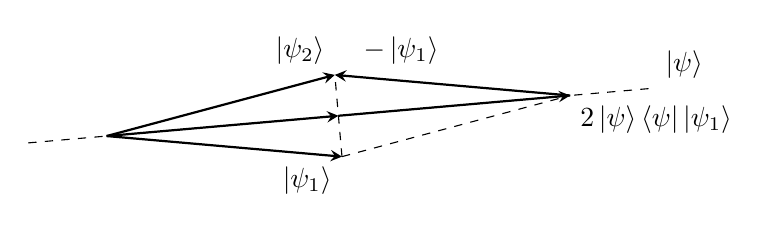
\begin{tikzpicture}[>=stealth]
                \draw[dashed] (-0.99619469809,-0.08715574274) -- (6.97336288664,0.61009019923)
                node[above right] {$\ket{\psi}$};
                \draw[dashed] (2.9885,-0.26146) -- (2.89777747887,0.7764571353);
                \draw[dashed] (2.9885,-0.26146) -- (5.88619591729,0.51497541405);
                \draw[->,thick] (0,0) -- (2.9885,-0.26146)
                node[below left] {$\ket{\psi_1}$};
                \draw[->,thick] (0,0) -- (2.89777747887,0.7764571353)
                node[above left] {$\ket{\psi_2}$};
                \draw[->,thick] (0,0) -- (2.94309795864,0.25748770702);
                \draw[->,thick] (2.94309795864,0.25748770702) -- (5.88619591729,0.51497541405)
                node[below right] {$2\ket{\psi}\bra{\psi} \ket{\psi_1}$};
                \draw[->,thick] (5.88619591729,0.51497541405) -- (2.89777747887,0.7764571353)
                node[above right] {$\ \ -\ket{\psi_1}$};
            \end{tikzpicture}
            \caption{Difusor equivale a uma reflexão em relação $\ket{\psi}$.}
        \end{figure}
        }
    \end{frame}

    \begin{frame}{Primeira Aplicação de $G$}
        \begin{figure}
            \centering
            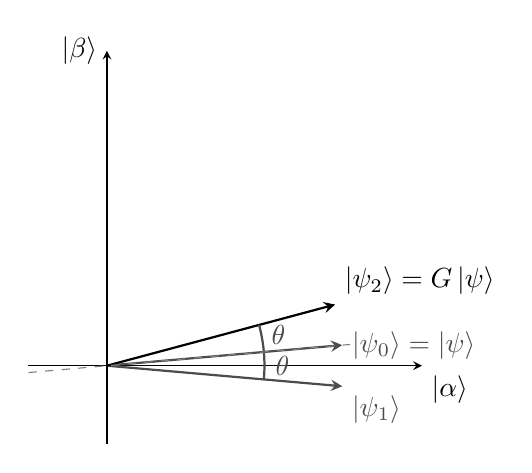
\begin{tikzpicture}[>=stealth]
                \draw[->] (-1,0) -- (4,0)
                node[below right] {$\ket{\alpha}$};
                \draw[->] (0,-1) -- (0,4)
                node[left] {$\ket{\beta}$};
%                \draw[gray,dashed] (-0.520944533,-2.95442325904) arc (-100:100:3);
                \draw[->,thick,black!70] (0,0) -- (2.9885,0.26146); %\psi_0
                \draw[->,thick,black!70] (0,0) -- (2.9885,-0.26146); %\psi_1
                \draw[->,thick] (0,0) -- (2.89777747887,0.7764571353); %\psi_2
                \draw[thick][black!70]  (1.99238939618,-0.17431148549) arc (-5:5:2);
                \draw[thick][black!70]  (1.99238939618,0.17431148549) arc (5:15:2);
                \draw[gray,dashed] (-0.99619469809,-0.08715574274) -- (3.08820356408,0.27018280251);
                % rótulos
                \draw[black!70] (2.9885,0.26146) node[right] {$\ket{\psi_0} = \ket{\psi}$};
                \draw[black!70] (2.9885,-0.26146) node[below right] {$\ket{\psi_1}$};
                \draw (2.89777747887,0.7764571353) node[above right] {$\ket{\psi_2} = G \ket{\psi}$};
                \draw[black!70] (2.1,0) node[right,inner sep=1pt] {$\theta$};
                \draw[black!70]  (2.05,0.39) node[right,inner sep=1pt] {$\theta$};
            \end{tikzpicture}
            \caption{Aplicar $G$ equivale à rotação de $\theta$ no sentido anti-horário.}
            \label{fig:first-grover}
        \end{figure}
    \end{frame}

    \begin{frame}{Aplicações Sucessivas de $G$}
        \begin{figure}
            \centering
            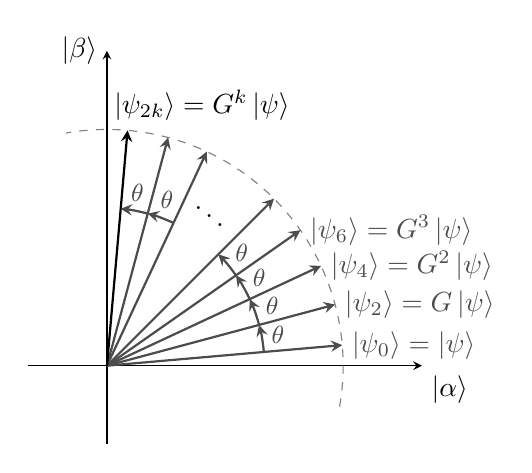
\begin{tikzpicture}[>=stealth]
                \draw[->] (-1,0) -- (4,0)
                node[below right] {$\ket{\alpha}$};
                \draw[->] (0,-1) -- (0,4)
                node[left] {$\ket{\beta}$};
                \draw[gray,dashed] (2.954,-0.5209) arc (-10:100:3);
                \draw[->,thick][black!70] (0,0) -- (2.9885,0.26146); %\psi_0
                \draw[->,thick][black!70] (0,0) -- (2.89777747887,0.7764571353); %\psi_2
                \draw[rotate around={25:(0,0)},->,thick][black!70] (0,0) -- (3,0); %\psi_4
                \draw[rotate around={35:(0,0)},->,thick][black!70] (0,0) -- (3,0); %\psi_6
                \draw[rotate around={45:(0,0)},->,thick][black!70] (0,0) -- (3,0); %\psi_8
                \draw[rotate around={65:(0,0)},->,thick][black!70] (0,0) -- (3,0); %\psi_{2(k-2)}
                \draw[rotate around={75:(0,0)},->,thick][black!70] (0,0) -- (3,0); %\psi_{2(k-1)}
                \draw[rotate around={85:(0,0)},->,thick] (0,0) -- (3,0); %\psi_{2k}
                %\draw[thick,black!70,->] (2,0) arc (0:5:2);
                \draw[rotate around={5:(0,0)},thick,black!70,->] (2,0) arc (0:10:2);
                \draw[rotate around={15:(0,0)},thick,black!70,->] (2,0) arc (0:10:2);
                \draw[rotate around={25:(0,0)},thick,black!70,->] (2,0) arc (0:10:2);
                \draw[rotate around={35:(0,0)},thick,black!70,->] (2,0) arc (0:10:2);
                \draw[rotate around={65:(0,0)},thick,black!70,->] (2,0) arc (0:10:2);
                \draw[rotate around={75:(0,0)},thick,black!70,->] (2,0) arc (0:10:2);
                % rótulos
                \draw[black!70] (2.9885,0.26146) node[right] {$\ket{\psi_0} = \ket{\psi}$};
                \draw[black!70] (2.89777747887,0.7764571353) node[right] {$\ket{\psi_2} = G \ket{\psi}$};
                \draw[black!70] (2.71892336111,1.26785478522) node[right] {$\ket{\psi_4} = G^2 \ket{\psi}$};
                \draw[black!70] (2.45745613287,1.72072930905) node[right] {$\ket{\psi_6} = G^3 \ket{\psi}$};
                \draw[rotate around={85:(0,0)}] (3,0) node[above right] {$\!\!\!\!\!\ket{\psi_{2k}} = G^k \ket{\psi}$};
                \draw (1.3,2) node {$\ddots$};
                %\draw[black!70] (2.1,-0.1) node[right,fill=white,inner sep=1pt] {\small $\theta/2$};
                \draw[black!70]  (2.05,0.39) node[right,inner sep=1pt] {\small $\theta$};
                \draw[rotate around={10:(0,0)},thick,black!70] (2.2,0.39) node[inner sep=1pt] {\small $\theta$};
                \draw[rotate around={20:(0,0)},thick,black!70] (2.2,0.39) node[inner sep=1pt] {\small $\theta$};
                \draw[rotate around={30:(0,0)},thick,black!70] (2.2,0.39) node[inner sep=1pt] {\small $\theta$};
                \draw[rotate around={60:(0,0)},thick,black!70] (2.2,0.39) node[inner sep=1pt] {\small $\theta$};
                \draw[rotate around={70:(0,0)},thick,black!70] (2.2,0.39) node[inner sep=1pt] {\small $\theta$};
            \end{tikzpicture}
            \caption{Aplicações sucessivas de $G$.}
            \label{fig:k-grover}
        \end{figure}
    \end{frame}

    \begin{frame}{Acerto, $k$ e $\theta$}
        \[
        \begin{matrix}
            k       &=& \dfrac{\pi}{4} \sqrt{\dfrac{N}{M}}      \\ \\
            \theta  &=& \arccos\left(\dfrac{N - 2}{N}\right)    \\ \\
            P_a     &=& \dfrac{N - 1}{N}
        \end{matrix}
        \]
    \end{frame}

    \begin{frame}{Ket vs Qiskit}
        \begin{table}
            \begin{tabular}{c | c}
                Ket                         &   Qiskit                  \\
                \hline \hline
                \pause
                $\ket{q_0 \dots q_n}$       &   $\ket{q_n \dots q_0}$   \\
                \pause
                \mintinline{python}{H(qubits)}      &   \mintinline{python}{qc.h(qubits)}\\
                \pause
                \mintinline{python}{ctrl()}         &   \mintinline{python}{qc.mcx()}
            \end{tabular}
            \label{tab:table}
        \end{table}
    \end{frame}

    \begin{frame}{Ket vs Qiskit: Código}
        \only<1>{
        \inputminted[
            bgcolor=lightgray,
            firstline=13,
            lastline=16
        ]{python}{src/grover/grover_ket.py}
        }
        \only<2>{
        \inputminted[
            bgcolor=lightgray,
            firstline=9,
            lastline=26
        ]{python}{src/grover/grover.py}
        }
        \only<3>{
        \inputminted[
            bgcolor=lightgray,
            firstline=19,
            lastline=26
        ]{python}{src/grover/grover_ket.py}
        }
        \only<4>{
        \inputminted[
            bgcolor=lightgray,
            firstline=29,
            lastline=41
        ]{python}{src/grover/grover.py}
        }
    \end{frame}

    \begin{frame}{Parâmetros dos Testes}
        \begin{itemize}
            \item 100 replicações.
            \item $n$ qubits, $n \in [2, 20)$.
            \item 1 estado aleatório marcado.
        \end{itemize}
    \end{frame}

    \begin{frame}{Tempo de Execução}
        \begin{figure}
            \begin{tikzpicture}
    \begin{axis}[
        xmin=2,
        ymin=0,
        ymax=10,
        xlabel={Nº Qubits},
        ylabel={Time (s)},
        legend pos=north west,
        legend entries={qubox, local, qubox-pbwd, qiskit-aer}]
        \addplot table [x=qubits, y=average] {dat/grover/ket_qubox_01.dat};
        \addplot[mark=*] table [x=qubits, y=average] {dat/grover/ket_local_01.dat};
        \addplot[mark=square*] table [x=qubits, y=average] {dat/grover/ket_qubox_pbwd_01.dat};
        \addplot[mark=triangle*] table [x=qubits, y=average] {dat/grover/qiskit_aer_01.dat};
    \end{axis}
\end{tikzpicture}
            \label{fig:execution-time}
        \end{figure}
    \end{frame}

    \begin{frame}{Precisão}
        \begin{figure}
            \only<1>{
            \precision{2}{5}
            }
            \only<2>{
            \precision{6}{9}
            }
            \only<3>{
            \precision{10}{13}
            }
            \only<4>{
            \precision{14}{17}
            }
            \label{fig:precision}
        \end{figure}
    \end{frame}
\end{document}